% Techfak Presentation template
% Developed by Benjamin Paaßen, 2019
%
% This LaTeX template is loosely based on the 2019 Bielefeld University Corporate Design
% https://www.uni-bielefeld.de/corporatedesign/
%
% It is developed from an earlier CITEC corporate design presentation template,
% also developed by Benjamin Paaßen
%
% For further question, you may contact me at https://bpaassen.gitlab.io/
%
% For this file to compile you need several other files, which should be part of
% any distribution of this file, namely:
%
% tango-colors.sty
% techfak_logo.pdf
% techfak_presentation_preamble.tex
% unibi-colors.sty

\documentclass[compress, aspectratio=169]{beamer}
%\usepackage[colorlinks=true, urlcolor=blue]{hyperref}
\hypersetup{colorlinks=true, urlcolor=blue}
% Techfak Presentation template
% Developed by Benjamin Paaßen, 2019
%
% This LaTeX template is loosely based on the 2019 Bielefeld University Corporate Design
% https://www.uni-bielefeld.de/corporatedesign/
%
% It is developed from an earlier CITEC corporate design presentation template,
% also developed by Benjamin Paaßen
%
% For further question, you may contact me at https://bpaassen.gitlab.io/
%
% For this file to compile you need several other files, which should be part of
% any distribution of this file, namely:
%
% tango-colors.sty
% techfak_logo.pdf
% techfak_presentation_preamble.tex
% unibi-colors.sty

\usepackage[utf8]{inputenc}
\usepackage[T1]{fontenc}
\usepackage{graphicx}
\usepackage{amssymb}
\mode<presentation>

\usepackage{tikz}
\usepackage{svg}
% unibi/techfak Colors
\usepackage{unibi-colors}
% additional colors
\usepackage{tango-colors}

% tikz styles

\usetikzlibrary{shapes, arrows, backgrounds, intersections, decorations.pathreplacing}

\tikzstyle{point}=[circle, inner sep=0pt, minimum size=3mm, thick, anchor=center]
\tikzstyle{textnode}=[draw=none, fill=none]
\tikzstyle{proto}=[diamond, inner sep=0pt, minimum size=7mm, thick, anchor=center]
\tikzstyle{edge}=[->, >=stealth', shorten <=2pt, shorten >=2pt, auto, semithick]
\tikzstyle{class0color}=[aluminium6]
\tikzstyle{class0}=[draw=aluminium6, fill=aluminium4, text=aluminium6]
\tikzstyle{class1color}=[techfak-blue]
\tikzstyle{class1}=[draw=techfak-blue, fill=techfak-blue-bright, text=techfak-blue]
\tikzstyle{class2color}=[unibi-green]
\tikzstyle{class2}=[draw=unibi-green, fill=unibi-green-bright, text=unibi-green]

% Beamer setup

\setbeamercolor*{structure}{fg=techfak-blue}
\setbeamercolor{block title}{bg=white}
\setbeamercolor{block body}{bg=WhiteSmoke}
\setbeamercolor*{footline}{bg=techfak-blue,fg=techfak-blue}

\usecolortheme{orchid}
\setbeamertemplate{navigation symbols}{}
\setbeamertemplate{footline}[frame number]{}
\setbeamertemplate{headline}{
% include techfak logo on every slight in the top right corner
\begin{tikzpicture}
\node at (0,0.2) {}; % anchor node
\node[right] at (13,-0.55) {
\includegraphics[width=2.5cm]{techfak_logo.pdf}}; % image node
\end{tikzpicture}

\vspace{-1.3cm}
}
\setbeamertemplate{frametitle}{
\usebeamerfont{frametitle}\usebeamercolor[fg]{frametitle}\insertframetitle
}
\setbeamertemplate{bibliography item}[text]
\setbeamertemplate{section in toc}[sections numbered]

\usefonttheme{professionalfonts}

% Kapiteltrennfolie
\newcommand{\chapterframe}[1]{

\begin{frame}

\vfill
\centering
\vspace{-2.3cm}
\begin{huge}
\usebeamerfont{title}\usebeamercolor[fg]{title}#1
\end{huge}

\end{frame}
}

% section slides

\AtBeginSection[]{
\chapterframe{\insertsectionhead}
}

% Title Frame Makro

\newcommand{\titleframe}[1]{
{

\begin{frame}[plain]
\usebackgroundtemplate{}%
\begin{tikzpicture}[overlay, remember picture]
% helper nodes
\node[anchor=center] (center) at (current page.center) {};
% actual picture
\node[anchor=center] (pic) [below of=center, node distance=0cm] {
\includegraphics[width=\paperwidth]{CodeFor-bielefeld.svg}%
};
\end{tikzpicture}
\end{frame}
}
}

% Picture frame makro

% Arguments:
% 1: Frame title
% 2: Image link
% 3: Image parameters
% 4: Copyright notice
\newcommand{\custompicframe}[4]{
\begin{frame}{#1}
\begin{tikzpicture}[overlay, remember picture]
% helper nodes
\node[anchor=south] (bottom) at (current page.south) {};
\node[anchor=center] (center) at (current page.center) {};
% actual picture
\node[anchor=center] (pic) [below of=center, node distance=0.5cm] {
\includegraphics[#3]{CodeFor-bielefeld.svg}%
};
% copyright notice
\node (copyright) [above of=bottom, node distance=0.6cm] {\color{techfak-blue-bright}\tiny #4};
\end{tikzpicture}
\end{frame}
}

% Arguments:
% 1: Image Name
% 2: Image Link
% 3: License Name
% 4: License Link
\newcommand{\cprtext}[4]{
{\color{techfak-blue-bright}\tiny #1 (\href{#2}{Link}); Usage according to \href{#4}{#3}.}
}

% Arguments:
% 1: Frame title
% 2: Image link
% 3: Image parameters
% 4: Image Name
% 5: Image Link
% 6: License Name
% 7: License Link
\newcommand{\picframe}[7]{
\custompicframe{#1}{#2}{#3}{#4 (\href{#5}{Link}); Usage according to \href{#7}{#6}.}
}

\setbeamercolor{alerted text}{fg=techfak-blue}
\renewcommand{\emph}[1]{\textbf{\color{techfak-blue} #1}}


\usepackage[english]{babel}
\usepackage{csquotes}
\usepackage{amssymb,amsmath,array}
%\usepackage{graphicx}
\usepackage{latexsym}
\usepackage{times}
\usepackage{booktabs}
\usepackage{paralist}
\usepackage{subcaption}
\usepackage{longtable}
\usepackage{geometry}


\usepackage{epsfig}
\usepackage{calc}
\usepackage{amstext}
\usepackage{amsthm}
\usepackage{multicol}
\usepackage{pslatex}
\usepackage{apalike}
\usepackage{wrapfig}



\title{Generating Synthetic Genotypes using Diffusion
Models}




\author{\small Philip Kenneweg, Raghuram Dandinasivara, Xiao Luo,\\ Barbara Hammer, Alexander Schönhuth }

\institute{University Bielefeld}

\hypersetup{
  pdftitle={My first Techfak presentation},
  pdfauthor={Martha McFirstAuthor},
  pdfkeywords={Science, LaTeX, Beamer, Presentation, Template}
}



\begin{document}


\begin{frame}[plain] % [plain] often looks better for title pages (removes header/footer)
    \titlepage
\end{frame}

% \begin{frame}{Unifying Data Modalities}
%     \begin{figure}
%         \centering
%         \includegraphics[width=0.8\linewidth]{figures/Title Background.png}
%     \end{figure}
% \end{frame}

\begin{frame}{Why do we need Synthetic Data?}


  \begin{columns}
\begin{column}{0.48\textwidth}
    \begin{itemize}
  \item Large high quality datasets are becoming available but getting access is a long and costly process (for example UKBB \footnote[frame]{\tiny  UK Biobank – cohort of ~ 500 000 participants with extensive health, genetic and imaging data. “About our data” page, UK Biobank. \url{https://www.ukbiobank.ac.uk/enable-your-research/about-our-data}. })
   \item High quality synthetic data would allow genomics data to be freely distributed (i.e. Kaggle dataset) without privacy concerns. 

  \end{itemize}
\end{column}
\begin{column}{0.48\textwidth}
\begin{figure}
    \centering
    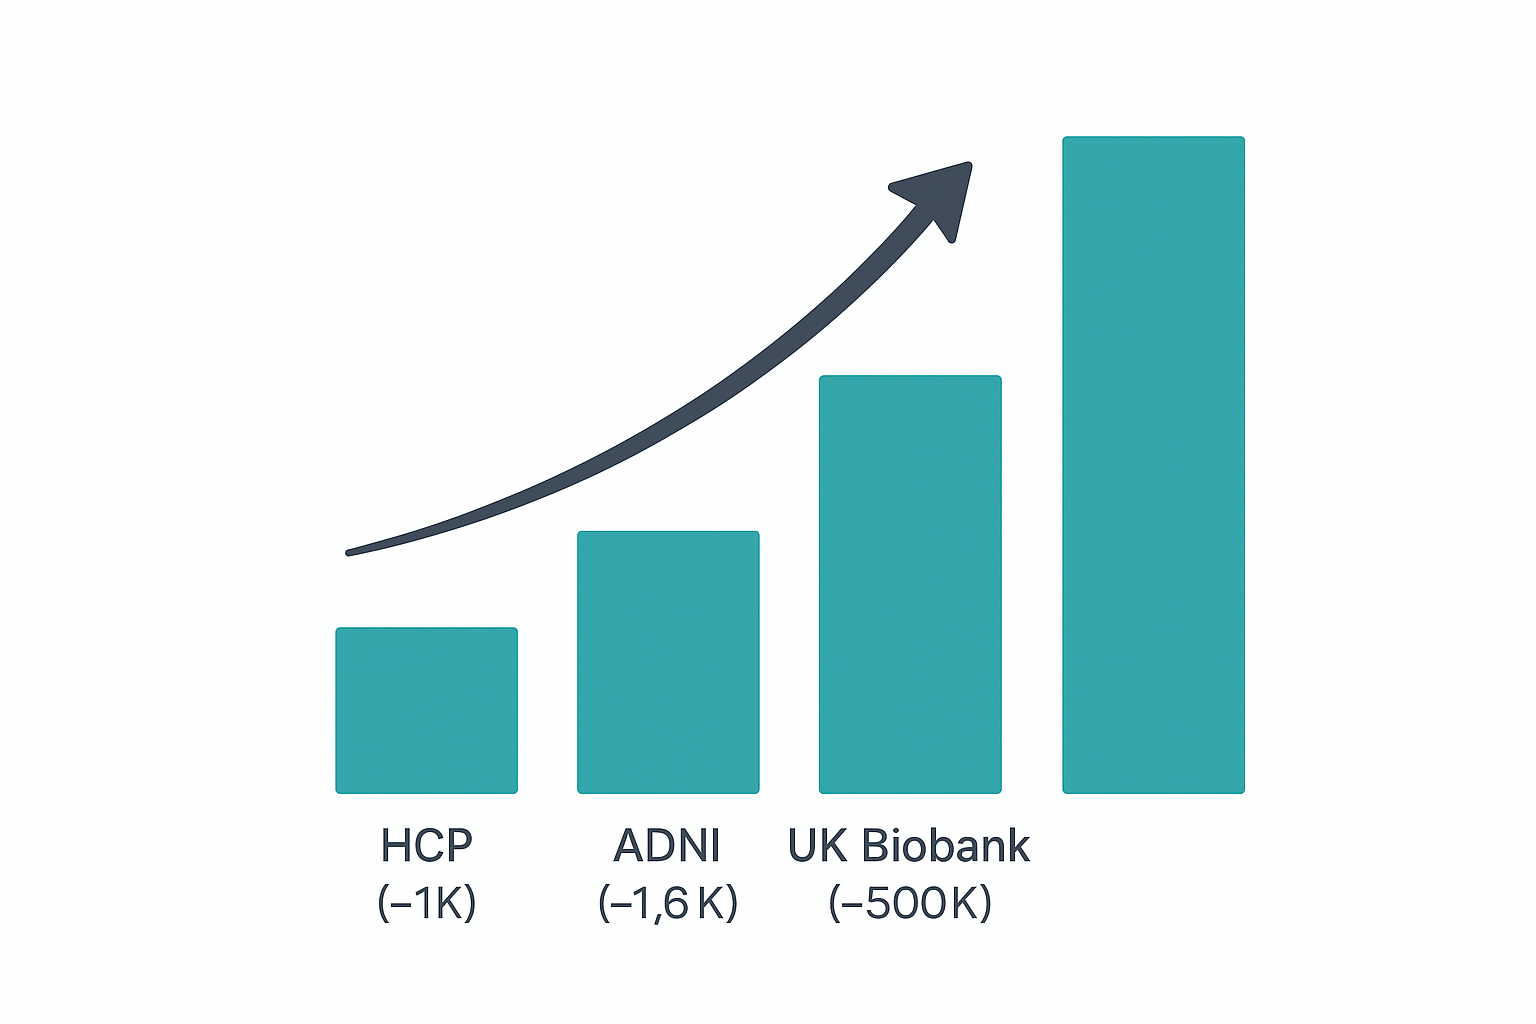
\includegraphics[width=0.8\linewidth]{figures/dataset_growth.png}
    \caption{\small Increasing availability of large scale genomics datasets.}
    
\end{figure}
\end{column}

  \end{columns}

 

\end{frame}

\begin{frame}{Possible Generative Models}
\begin{multicols}{2}
\begin{itemize}
    \item Variational Autoencoder
    \item Generative Adversarial Networks
    \item Generative Markov Models
    \item Diffusion Models
    \item Autoregressive Models (LLM Style)
\end{itemize}
\columnbreak

\begin{figure}
    \centering
    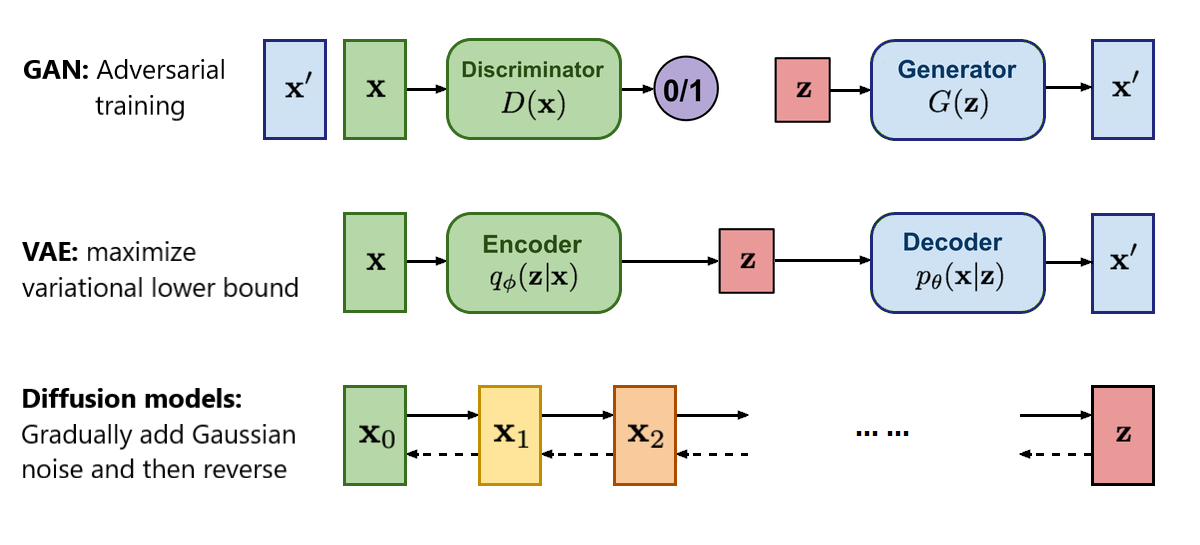
\includegraphics[width=1.0\linewidth]{figures/generativemodels.png}
\end{figure}
\end{multicols}

\end{frame}

\begin{frame}{Possible Generative Models}
\begin{itemize}
    \item Variational Autoencoder - Output quality not state of the art, does not scale well, ...
    \item Generative Adversarial Networks - Unstable, hard to train, ...
    \item Generative Markov Models - Not very powerfull or general, ...
\end{itemize}
\end{frame}

\begin{frame}{Possible Generative Models}

\begin{multicols}{2}
\begin{itemize}
    \item Diffusion Models - best suited for fixed length generation with causal interactions in all directions, can produce very high quality output by refining over multiple passes
    \item Autoregressive Models (LLM Style) - best suited for non-fixed length with causal interactions left to right, produces good output, mostly used for high level tasks
\end{itemize}

Genome has interactions in all directions, fixed length, high quality needed \newline -> Diffusion Models

\columnbreak

\begin{figure}
    \centering
    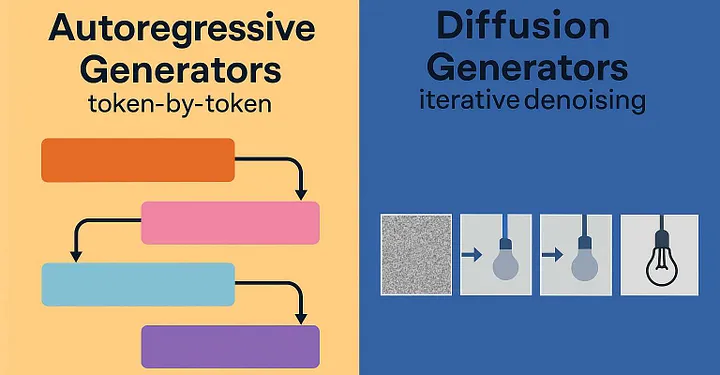
\includegraphics[width=1.0\linewidth]{figures/autovsdiff.png}
\end{figure}
\end{multicols}

\end{frame}

\begin{frame}{Related Work}
    \small
\begin{table}
  \centering
  \caption{An overview of related work on generating synthetic genomes and its differences / similarities in comparison with our work. Our novelties are \textbf{highlighted}.}
  \label{Fig:overviewrelated}
  \begin{tabular}{c|cccc}
    \toprule
Reference & Model & Data Type & Genome Length  & Cond. \\
 
   \cmidrule(r){1-5} 

DNAGPT \cite{zhang2023dnagpt}& Autoregressive & Base-Pairs & 24k BPS &  x \\
HyenaDNA \cite{nguyen2023hyenadna} & Autoregressive & Base-Pairs & $10^6$ BPS & x\\
HAPNEST \cite{hapnest} & LD \& Markov & SNPs & 1 Chromosome   & x \\
\cite{perera2022generative} & GMMNs & SNPs & 1 Chromosome & \checkmark\\
\cite{yelmen2021creating} & GAN,RBM & SNPs & 10k SNPs &  x\\
\cite{yelmen2023deep} & WGAN & SNPs & 10k SNPs  &  x\\
\cite{szatkownik2024towards} & WGAN  & PCA+SNPs & 65k SNPs & x \\
\cite{ahronoviz2024genome} &  GAN & SNPs & 10k SNPs &  \checkmark \\
\cite{burnard2023generating} & VAE & SNPs & 1 Chromosome & x \\
\cite{dang2023tractable} &  HCLTs  & SNPs & 10k SNPs & x \\
%\cite{Geleta2023.09.27.558320} & VQ-VAE & SNPs & 10k SNPs & \checkmark \\
GeneticDiffusion (Ours) & \textbf{Diffusion} & PCA+SNPs & \textbf{Full Genome} &   \checkmark \\
    \bottomrule
  \end{tabular}
\end{table}
\end{frame}

\begin{frame}{Pre-Processing}
    \begin{figure}
    \centering
    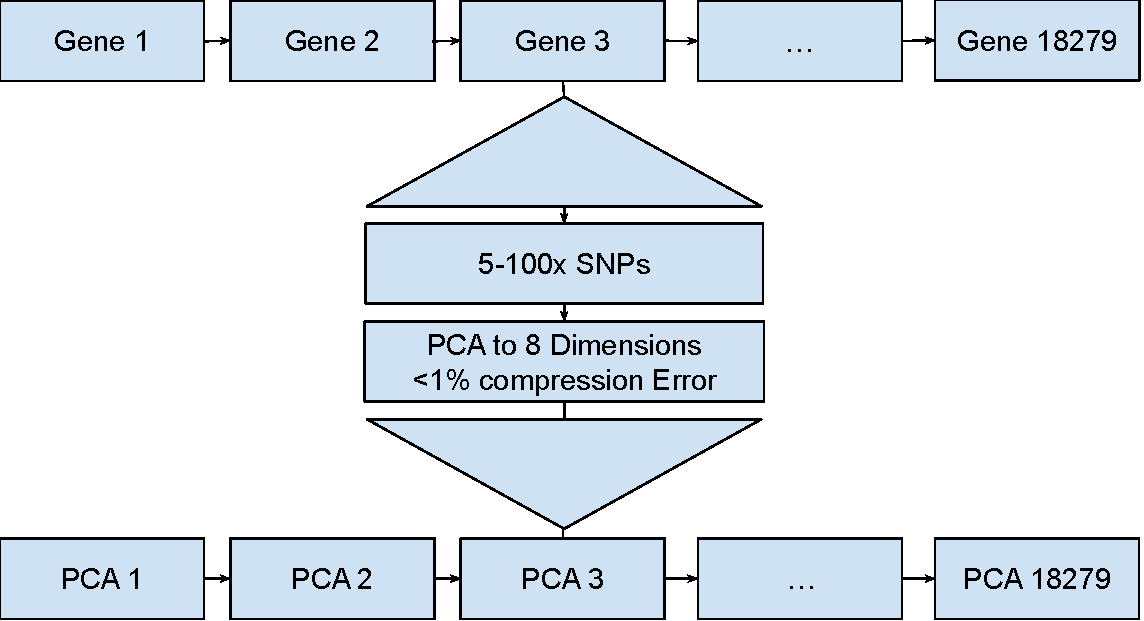
\includegraphics[width = 0.65\textwidth]{figures/Kenneweg.141.fig.1.pdf}
    \caption{Overview of the Pre-processing pipeline. Genes, which consist of between 5 to 100 SNPs are each processed by a custom PCA. This is done independently for each Gene.}
    \label{fig:pca}
\end{figure}

\end{frame}

\begin{frame}{Model Architecture}
\begin{multicols}{2}  
Possible options:
    \begin{itemize}
        \item Transformer - No spatial bias, popular, needs high amount of training data
        \item U-Net CNN - Local spatial bias, few parameters
        \item U-Net MLP - Overfits easily, hard to train
        \item Combinations are also possible
    \end{itemize}
\columnbreak

\begin{figure}
    \centering
    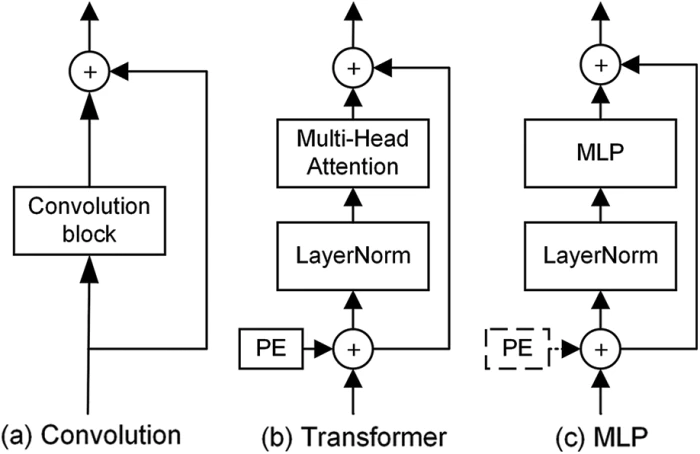
\includegraphics[width=1.0\linewidth]{figures/architecture.png}
\end{figure}
\end{multicols}

\end{frame}

\begin{frame}{Model Architecture}
\begin{figure}
    \centering
     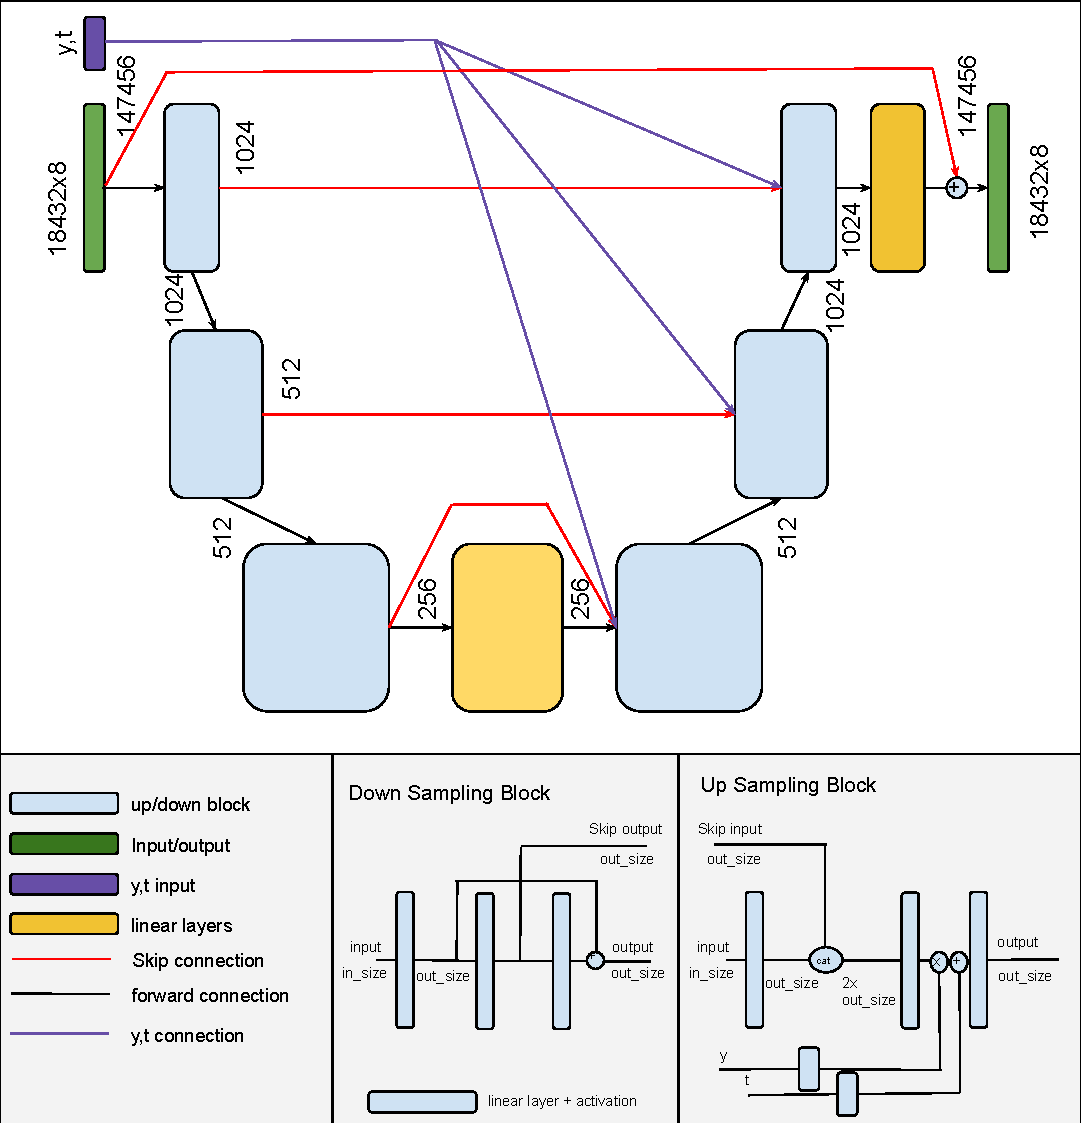
\includegraphics[width = 0.48\textwidth]{figures/Kenneweg.141.fig.2.pdf}
    \caption{A structural overview of the architecture of the MLP diffusion model.}
    \label{fig:unet}
\end{figure}
\end{frame}

\begin{frame}{Evaluation}
\begin{multicols}{2}
    We evaluate on 2 different classification tasks: 
\begin{itemize}
    \item ALS classification
    \item 1KG region classification
\end{itemize}

Recovery Rate compares the performance of the syn model $a_s$ vs the true model $a_r$:
\begin{equation}
    R(a_r,a_s) = \frac{a_s}{a_r}
\end{equation}
    \columnbreak
\begin{figure}
    \centering
     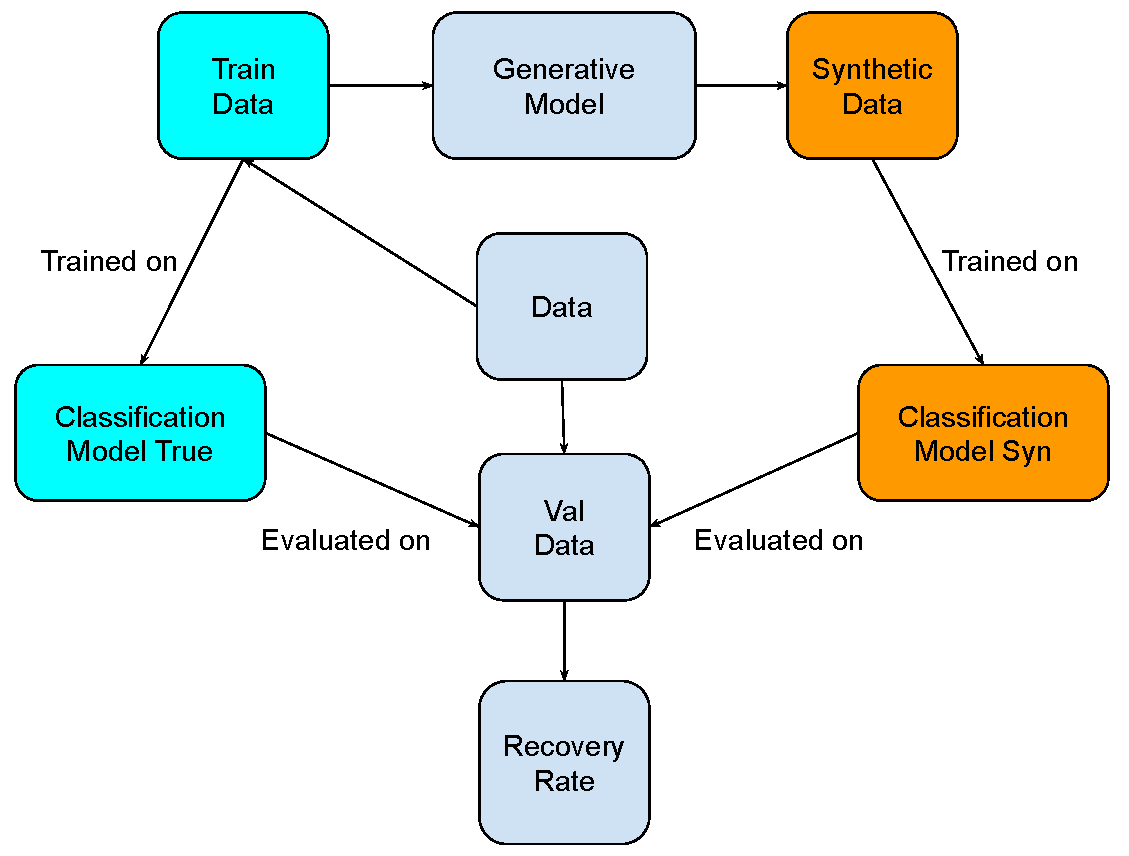
\includegraphics[width = 0.48\textwidth]{figures/Recovery Rate.pdf}
    \caption{A diagram of the evaluation pipeline.}
    \label{fig:unet}
\end{figure}
\end{multicols}


\end{frame}

\begin{frame}{Evaluation}
\begin{multicols}{2}
Additional metric: 

Nearest Neighbour Adversarial Accuracy \cite{yale2019privacy} - relies on distances of generated samples to original samples.
\bigbreak
Problem: 

Distances/neighbourhood in high dimensional space are not inherently meaningful \cite{beyer1999nearest}.
\columnbreak

\begin{figure}
    \centering
    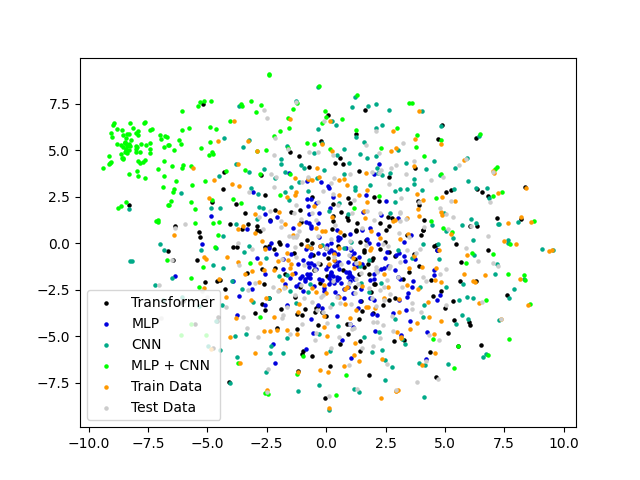
\includegraphics[width=1.0\linewidth]{figures/umap_mlp_euclidean.png}
\end{figure}
\end{multicols}


    
\end{frame}

\begin{frame}{Experiments}

We evaluated 4 different generative architectures:

\begin{itemize}
    \item MLP
    \item CNN
    \item MLP + CNN
    \item Transformer
\end{itemize}

The metrics we used: 

\begin{itemize}
    \item Recovery Rate
    \item Nearest Neighbour Adversarial Accuracy
    \item Accuracy improvement with partial synthetic data
\end{itemize}
    
\end{frame}


\begin{frame}{Results Recovery Rate}


\begin{table}[ht!]
  \centering
  \caption{Recovery rates on a hold out test set of true genotypes after training different ALS or 1KG population classifiers (MLP, Transformer or CNN)  on different synthetically generated data types (generated by: MLP, Transformer, CNN, MLP + CNN). The best synthetic data for each classifier type is marked in \textbf{bold}.}
  \label{Fig:cls}
  \begin{tabular}{c|cccc}
    \toprule
Classifier & CNN  & MLP  & MLP+CNN & Transformer \\ %todo uptade mlp+cnn
 
   \cmidrule(r){1-5} 
  & & ALS data  \\
MLP &   71.51 & \textbf{96.69} & 94.26 & 73.77 \\
Transformer &  66.06 & 93.44 & \textbf{93.89} & 69.30 \\
CNN & 69.88 & 91.72 & \textbf{93.17} & 68.72 \\
\cmidrule(r){1-5} 
& &1KG data \\
 MLP &   15.58 & 65.80 & \textbf{93.02} & 13.28 \\
  Transformer &  16.23 & 62.99 & \textbf{84.98} & 8.38 \\
 CNN &   19.52 & 56.57 & \textbf{77.54} & 21.21 \\
\cmidrule(r){1-5} 
 Average (all) & 43.17 & 78.06 & \textbf{89.48} & 42.56\\
    \bottomrule
  \end{tabular}
\end{table}
    
\end{frame}

\begin{frame}{Results NNAA}
    \small
\begin{table}
 % \vspace{+0.05\textwidth}
  \centering
  \caption{Result of Nearest Neighbour Adversarial Accuracy for generated datasets on the ALS and 1KG data; For AA the closer to 0.5 the better, For Privacy Loss the closer to 0 the better; best performance is \textbf{highlighted}.}
  \label{Fig:nnaccals}
  \begin{tabular}{c c c | cccc}
    \toprule
& &  & CNN & MLP  & MLP + CNN & Transformer  \\

  \cmidrule(r){1-3}  \cmidrule(r){3-7} 
 ALS data &test data &  $AA_{truth}$ & 0.735 & 0.255  & \textbf{0.485} & 0.92 \\
& &  $AA_{syn}$&0.68 & 1.0  & 0.93 &   \textbf{0.66}  \\
  % $AA_{TS}$ & 0.7075 & 0.6275  & 0.7075  & 0.79 \\
  \cmidrule(r){2-3}  \cmidrule(r){3-7}
 & train data & $AA_{truth}$ & 0.81 & 0.005  & \textbf{0.405} & 0.93 \\
 & & $AA_{syn}$& \textbf{0.67} & 1.0  & 0.92 &  0.69  \\
  % $AA_{TS}$ & 0.74 & 0.5025  & 0.66  & 0.81 \\
  \cmidrule(r){2-3}  \cmidrule(r){3-7}
 & & Privacy Loss & 0.0325 & 0.125 & 0.0475 & \textbf{0.02} \\


  \cmidrule(r){1-3}  \cmidrule(r){3-7} 
1KG data  &test data &  $AA_{truth}$ & 0.76 & 0.0  & \textbf{0.63} & 0.345 \\
& &  $AA_{syn}$& 0.995 & 1.0  & 0.94 & \textbf{0.92}  \\
  % $AA_{TS}$ & 0.8775 & 0.5  & 0.785  & 0.6325 \\
  \cmidrule(r){2-3}  \cmidrule(r){3-7}
& train data & $AA_{truth}$ & 0.765 & 0.0 & \textbf{0.385} & 0.285 \\
 & & $AA_{syn}$& 1.0 & 0.99  & \textbf{0.74} &  0.82 \\
  % $AA_{TS}$ & 0.8825 & 0.495  & 0.5625  & 0.5525 \\
  \cmidrule(r){2-3}  \cmidrule(r){3-7}
 & & Privacy Loss & 0.05 & \textbf{-0.005} & -0.2225 & 0.08 \\

    \bottomrule
  \end{tabular}
\end{table}
\end{frame}

\begin{frame}{Partial Synthetic and Real}

  \begin{figure}
    \centering
    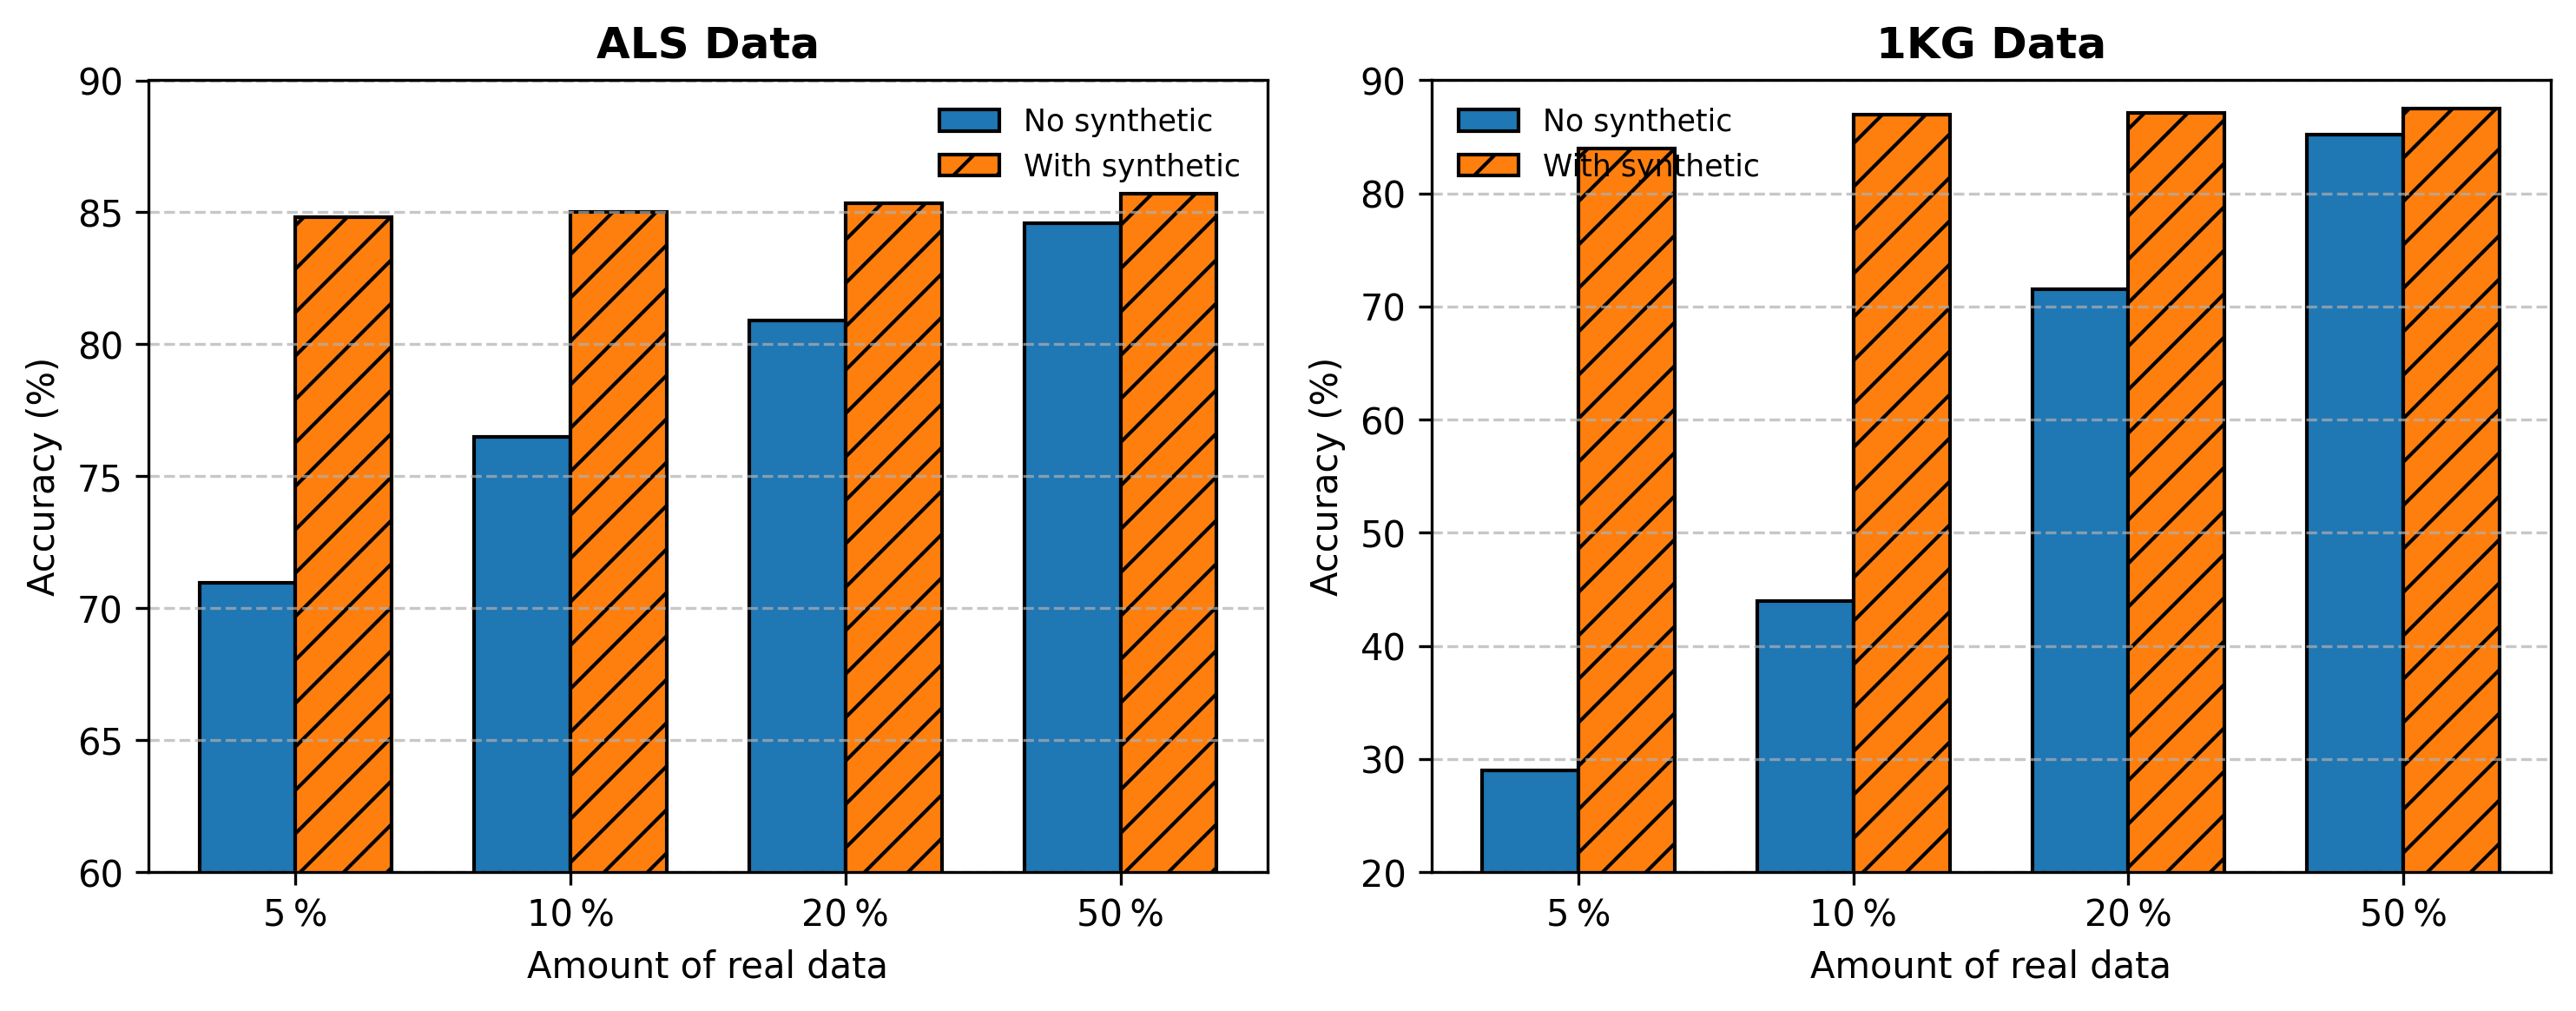
\includegraphics[width=0.8\textwidth]{figures/synimpro.png}
    \caption{Accuracy improvements by integration of synthetic data for best performing classification architecture.}
    \label{Fig:potimprove}
  \end{figure}
    
% \begin{table}[h!]
%   \centering
%   \caption{Accuracy improvements by integration of best synthetic data for best performing classification architecture.}
%   \label{Fig:potimprove}
%   \begin{tabular}{cl|cccc}
%     \toprule
% & amount real data & 5\% & 10\% & 20\% & 50\%  \\
 
%    \cmidrule(r){1-6} 
% ALS Data & no syn data &  70.96  & 76.50 & 80.90 & 84.60   \\
% & with syn data & 84.83 & 85.01 & 85.34  & 85.70  \\

%    \cmidrule(r){1-6} 
% 1KG data & no syn data &  29.01 & 43.99 & 71.52 & 85.19  \\
% & with syn data & 83.98 & 86.93 & 87.11 & 87.50   \\
%     \bottomrule
%   \end{tabular}
% \end{table}
\end{frame}

\begin{frame}{Conclusion}
\begin{itemize}
    \item Synthetic data does not just copy real data, while close to real data distribution (see NNAA)
    \item Recovery Rate indicates high fidelity of synthetic data.
\end{itemize}
\bigbreak
Next Steps:
\begin{itemize}
    \item Bigger dataset (for example UK Biobank)
    \item Multimodal data
    \item Publish synthetic dataset
\end{itemize}

    
\end{frame}
% Slide 13: Q & A
\begin{frame}{Q \& A}
    \textbf{Questions and Discussion}
    

    \textit{Feel free to ask anything.}
\end{frame}


\section{Bibliography}
\tiny
\bibliography{reference}
\bibliographystyle{apalike}

\end{document}

% I usually don't want to include the literature slides and backup slides into the slide numbering
% for the actual talk, so I use this little trick.
\newcounter{lastframeidx}
\setcounter{lastframeidx}{\value{framenumber}}



\setcounter{framenumber}{\value{lastframeidx}}

\end{document}
